% !TEX root = ../discretemath.tex

\section{Функция Мёбиуса ЧУМ. Свойства произведения ЧУМов}

\subsection{Частично упорядоченные множества}

\begin{Definition}{Частично упорядоченное множество (ЧУМ)}{}
	Множество $P$ с отношением строгого порядка $<$ — \emph{ЧУМ}, если выполнены:
	\begin{enumerate}
		\item \textbf{Иррефлексивность:} $x\not<x$;
		\item \textbf{Антисимметричность:} $x<y$ и $y<x$ одновременно невозможны;
		\item \textbf{Транзитивность:} $x<y$ и $y<z$ $\Rightarrow$ $x<z$.
	\end{enumerate}
	Пишем $x\le y$, если $x<y$ или $x=y$. Для $x\le y$ \emph{отрезок} — это $[x,y]=\{z\mid x\le z\le y\}$. Рассматриваем только локально конечные ЧУМы (каждый отрезок конечен).
\end{Definition}

\subsection{Функция Мёбиуса}

\begin{Definition}{Функция Мёбиуса ЧУМа}{}
	\emph{Функция Мёбиуса} $\mu\colon P\times P\to\mathbb Z$ задаётся рекурсивно:
	\[
	\mu(x,y)=
	\begin{cases}
		1, & x=y,\\[4pt]
		-\displaystyle\sum_{x\le z<y}\mu(x,z), & x<y,\\[6pt]
		0, & \text{иначе.}
	\end{cases}
	\]
\end{Definition}

\begin{Corollary}{Эквивалентное определение}{}
	$\mu$ задаётся условиями
	\[
	\mu(x,x)=1,\qquad \sum_{x\le z\le y}\mu(x,z)=0 \text{ при } x<y.
	\]
	Действительно, $\mu(x,y)=-\sum_{x\le z<y}\mu(x,z)$ равносильно $\sum_{x\le z\le y}\mu(x,z)=0$.
\end{Corollary}

\begin{Remark}{}{}
	Функция Мёбиуса существует и единственна: при $x=y$ значение $1$, при $x\nleq y$ — $0$, а при $x<y$ значение однозначно выражается через $\mu(x,z)$ для $z<y$. Локальная конечность гарантирует, что все суммы конечны.
\end{Remark}

\subsection{Примеры}

\begin{Example}{Пятиэлементный ЧУМ}{}
	Множество $\{0,a,b,c,d\}$ с $0<a<d$ и $0<b<c<d$, где $a$ и $c$ несравнимы.

	\begin{center}
		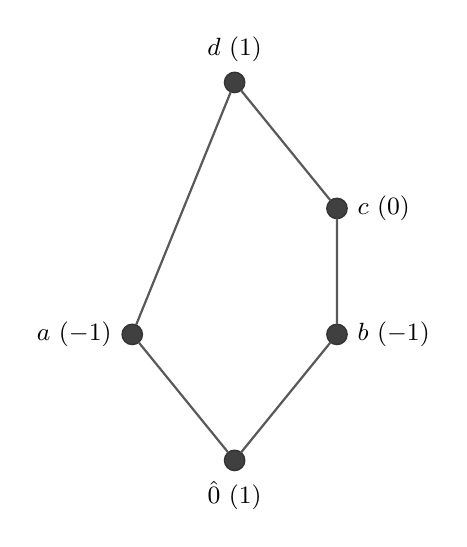
\begin{tikzpicture}[
			scale=1,
			nd/.style={circle, draw=black!80, fill=black!75, inner sep=2.6pt, line width=0.5pt},
			lbl/.style={font=\small},
			edge/.style={thick, draw=black!65, line cap=round}
			]
			\node[nd, label={[lbl]below:$\hat{0}\ (1)$}]   (bot) at ( 0.0, 0.0) {};
			\node[nd, label={[lbl]left:$a\ ({-1})$}]        (a)   at (-1.3, 1.6) {};
			\node[nd, label={[lbl]right:$b\ ({-1})$}]       (b)   at ( 1.3, 1.6) {};
			\node[nd, label={[lbl]right:$c\ (0)$}]          (c)   at ( 1.3, 3.2) {};
			\node[nd, label={[lbl]above:$d\ (1)$}]          (top) at ( 0.0, 4.8) {};
			\draw[edge] (bot)--(a)--(top);
			\draw[edge] (bot)--(b)--(c)--(top);
		\end{tikzpicture}
	\end{center}
	В скобках — значение $\mu(0,\cdot)$. Проверка:
	\begin{align*}
		\mu(0,0)&=1,\\
		\mu(0,a)&=-\mu(0,0)=-1,\\
		\mu(0,b)&=-\mu(0,0)=-1,\\
		\mu(0,c)&=-(\mu(0,0)+\mu(0,b))=-(1-1)=0,\\
		\mu(0,d)&=-(\mu(0,0)+\mu(0,a)+\mu(0,b)+\mu(0,c))=-(1-1-1+0)=1.
	\end{align*}
\end{Example}

\begin{Example}{Булева решётка $2^{\{1,\ldots,n\}}$}{}
	$P=2^{\{1,\ldots,n\}}$ — все подмножества, упорядоченные по включению: $A\le B\Leftrightarrow A\subseteq B$.
\end{Example}

\begin{Theorem}{Функция Мёбиуса булевой решётки}{}
	В $2^{\{1,\ldots,n\}}$:
	\[
	\mu(A,B)=
	\begin{cases}
		(-1)^{|B|-|A|}, & A\subseteq B,\\
		0, & \text{иначе.}
	\end{cases}
	\]
\end{Theorem}

\begin{proof}
	Индукция по $|B\setminus A|$. \textbf{База:} $A=B$, $\mu(A,A)=1=(-1)^0$.

	\textbf{Переход:} пусть $A\subsetneq B$, $n=|B|-|A|$. По определению и ИП
	\[
	\mu(A,B)=-\sum_{A\subseteq C\subsetneq B}\mu(A,C)=-\sum_{A\subseteq C\subsetneq B}(-1)^{|C|-|A|}=-\sum_{k=0}^{n-1}(-1)^k\binom{n}{k},
	\]
	так как множеств $C$ с $|C|-|A|=k$ ровно $\binom{n}{k}$. Из $\sum_{k=0}^{n}(-1)^k\binom{n}{k}=(1-1)^n=0$ следует $\sum_{k=0}^{n-1}(-1)^k\binom{n}{k}=-(-1)^n$, поэтому
	\[
	\mu(A,B)=-(-(-1)^n)=(-1)^n=(-1)^{|B|-|A|}.
	\]
\end{proof}

\begin{figure}[H]
	\centering
	\begin{tikzpicture}[scale=1, font=\small,
		nd/.style={circle, draw, fill=black!8, inner sep=1pt, minimum size=14pt}]
		\node[nd] (e) at (0,0) {$\varnothing$};
		\node[nd] (1) at (-2,1.4) {$1$};
		\node[nd] (2) at (0,1.4) {$2$};
		\node[nd] (3) at (2,1.4) {$3$};
		\node[nd] (12) at (-2,2.8) {$12$};
		\node[nd] (13) at (0,2.8) {$13$};
		\node[nd] (23) at (2,2.8) {$23$};
		\node[nd] (123) at (0,4.2) {$123$};
		\draw (e)--(1) (e)--(2) (e)--(3);
		\draw (1)--(12) (1)--(13) (2)--(12) (2)--(23) (3)--(13) (3)--(23);
		\draw (12)--(123) (13)--(123) (23)--(123);
		\node[right=10pt, align=left] at (2.4,2.1)
		{$\mu(\varnothing,A)$:\\ $\varnothing\!:+1$\\ слой $1$: $-1$\\ слой $2$: $+1$\\ слой $3$: $-1$};
	\end{tikzpicture}
	\caption{Булева решётка $2^{\{1,2,3\}}$. Знак $\mu(\varnothing,A)=(-1)^{|A|}$ чередуется по слоям мощности: $+1,-1,+1,-1$. Это «решётчатый» аналог чередования знаков в формуле включений-исключений.}
\end{figure}

\subsection{Лемма о симметричной сумме}

\begin{Lemma}{}{}
	Для любых $x<y$ в ЧУМ $P$:
	\[
	\sum_{x\le z\le y}\mu(z,y)=0.
	\]
\end{Lemma}

\begin{proof}
	Индукция по $|[x,y]|$. \textbf{База:} $|[x,y]|=2$ (нет промежуточных): $\mu(x,y)+\mu(y,y)=-\mu(x,x)+1=0$.

	\textbf{Переход:} выделим $z=y$:
	\[
	\sum_{x\le z\le y}\mu(z,y)=\sum_{x\le z<y}\mu(z,y)+1.
	\]
	Подставив $\mu(z,y)=-\sum_{z\le u<y}\mu(z,u)$ и поменяв порядок суммирования:
	\[
	\sum_{x\le z<y}\mu(z,y)=-\sum_{x\le u<y}\sum_{x\le z\le u}\mu(z,u).
	\]
	Внутренняя сумма равна $1$ при $u=x$ (это $\mu(x,x)$) и $0$ при $x<u<y$ (по ИП, $[x,u]$ меньше). Значит,
	\[
	\sum_{x\le z\le y}\mu(z,y)=-(1+0+\dots+0)+1=0.
	\]
\end{proof}

\subsection{Двойственный ЧУМ}

\begin{Definition}{Двойственный ЧУМ}{}
	\emph{Двойственный} ЧУМ $P^*$ — то же множество с обратным порядком: $x\le^* y\Leftrightarrow x\ge y$ в $P$. Его функцию Мёбиуса обозначаем $\mu^*$.
\end{Definition}

\begin{Theorem}{Функция Мёбиуса двойственного ЧУМа}{}
	$\mu_P(a,b)=\mu^*(b,a)$.
\end{Theorem}

\begin{proof}
	Покажем, что $f(a,b):=\mu^*(b,a)$ удовлетворяет определяющим условиям $\mu_P$. Во-первых, $f(a,a)=\mu^*(a,a)=1$. Во-вторых, для $a<b$ в $P$ (то есть $b<^*a$ в $P^*$) по лемме о симметричной сумме в $P^*$:
	\[
	\sum_{a\le z\le b}f(a,z)=\sum_{a\le z\le b}\mu^*(z,a)=0.
	\]
	По единственности функции Мёбиуса $\mu_P(a,b)=\mu^*(b,a)$.
\end{proof}

\subsection{Прямое произведение ЧУМ}

\begin{Definition}{Прямое произведение}{}
	Для ЧУМов $A,B$ \emph{прямое произведение} $A\times B$ — ЧУМ на парах с покоординатным порядком:
	\[
	(a,b)\le(a',b')\Leftrightarrow a\le_A a'\text{ и }b\le_B b'.
	\]
\end{Definition}

\begin{Theorem}{Мультипликативность функции Мёбиуса}{}
	\[
	\mu_{A\times B}\bigl((a,b),(a',b')\bigr)=\mu_A(a,a')\cdot\mu_B(b,b').
	\]
\end{Theorem}

\begin{proof}
	Индукция по размеру интервала $[(a,b),(a',b')]$.

	\textbf{База:} $a=a'$ или $b=b'$. Если $a=a'$, то $[(a,b),(a,b')]\cong[b,b']$, откуда $\mu_{A\times B}=\mu_B(b,b')=\underbrace{\mu_A(a,a)}_{=1}\mu_B(b,b')$. Случай $b=b'$ симметричен.

	\textbf{Переход:} $a<a'$, $b<b'$. Из обнуления суммы в $A\times B$ и ИП для всех $(s,t)\neq(a',b')$:
	\begin{align*}
		\mu_{A\times B}\bigl((a,b),(a',b')\bigr)
		&=-\!\!\sum_{\substack{a\le s\le a',\,b\le t\le b'\\(s,t)\neq(a',b')}}\!\!\mu_A(a,s)\mu_B(b,t)\\
		&=\mu_A(a,a')\mu_B(b,b')-\Bigl(\sum_{a\le s\le a'}\mu_A(a,s)\Bigr)\Bigl(\sum_{b\le t\le b'}\mu_B(b,t)\Bigr)\\
		&=\mu_A(a,a')\mu_B(b,b')-0\cdot 0=\mu_A(a,a')\mu_B(b,b').
	\end{align*}
\end{proof}

\subsection{Формула обращения Мёбиуса}

\begin{Definition}{Обозначение $\hat\mu$}{}
	Если у $P$ есть минимальный элемент $\hat 0$, полагаем $\hat\mu(x):=\mu(\hat 0,x)$.
\end{Definition}

\begin{Theorem}{Формула обращения Мёбиуса}{}
	Пусть $P$ — ЧУМ с минимальным элементом $\hat 0$, $f,g\colon P\to\mathbb R$. Равносильны:
	\begin{enumerate}
		\item $f(x)=\displaystyle\sum_{z\le x}g(z)$ для всех $x$;
		\item $g(x)=\displaystyle\sum_{z\le x}\mu(z,x)f(z)$ для всех $x$.
	\end{enumerate}
\end{Theorem}

\begin{proof}
	\textbf{(1)$\Rightarrow$(2).} Подставим $f(z)=\sum_{y\le z}g(y)$:
	\[
	\sum_{z\le x}\mu(z,x)f(z)=\sum_{y\le x}\Bigl(\sum_{y\le z\le x}\mu(z,x)\Bigr)g(y).
	\]
	По лемме о симметричной сумме внутренняя сумма равна $1$ при $y=x$ и $0$ при $y<x$, поэтому всё равно $g(x)$.

	\textbf{(2)$\Rightarrow$(1).} Подставим $g(z)=\sum_{y\le z}\mu(y,z)f(y)$:
	\[
	\sum_{z\le x}g(z)=\sum_{y\le x}\Bigl(\sum_{y\le z\le x}\mu(y,z)\Bigr)f(y),
	\]
	и по обнулению суммы внутренняя сумма равна $1$ при $y=x$, $0$ иначе, откуда всё равно $f(x)$.
\end{proof}
